\section{Introduction}
Before we dive into our work, we briefly talk about our task and introduce the key concepts and models that we used during our project.
\subsection{Task}
The purpose of our task was to understand and implement NMT models and do a comparison between them and state-of-art models, to achieve that we had to build an encoder-decoder from scratch and then we exploited the transformers available on Hugginface.com \cite{huggingface_co} to improve the performance of our model. The best one was then pushed even further by feeding it more records during training and letting it run for more epochs in hope to achieve a better revisited BLEU score by \cite{goyal2021flores}. As for the datasets we used the english-italian one from \cite{anki_dataset} and the en-it europarl \cite{koehn2005europarl}, which, combined, resulted in more than 2 milion records, not enough to reach the perfomances of state-of-art models, but still useful to achieve nice results.
\vspace{3mm}

Over the next subsections, we'll talk about NMT and the models used for our work and their architecture, to give a better insight on their peculiarities and how we tried to exploit them.
\subsection{Neural Machine Translation}\label{subsec:NMT}
Neural Machine Translation, or simply NMT, is an approach to translate sentences from one language to another one (e.g.: from english to italian) by using a single neural network whose architecture is based on the encoder-decoder paradigm.
In its easiest form the network is composed by two RNNs (LSTMs or GRUs), one for the encoder and one for the decoder, that are trained jointly, in an end-to-end fashion, for maximizing the translation performance; such model composed of two RNNs has a very straight forward way of working:
\begin{itemize}
    \item The \textbf{encoder} receives one sentence from the source language and produces an encoding from it, such encoding will provide the fist hidden state of the decoder;
    \item The \textbf{decoder} receives the encoding produced by the encoder and builds the sentence in the target language one word at time conditioned on the encoding.
\end{itemize}
\begin{figure}[H]%
    \centering
    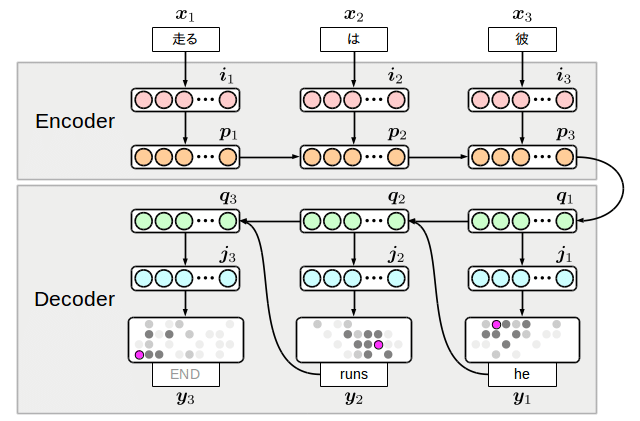
\includegraphics[width=0.65\linewidth]{images/seq2seq.png}
    \caption{Standard NMT model}
    \label{fig:NMT_model}
\end{figure}
This extremely simple model beat all the previous paradigms by a large margin providing more fluent and precise context-wise translations and its training was even easier since both parts, encoder and decoder, are trained together giving less headaches on optmizing every single sub-module.
\subsection{Transformer}\label{subsec:transformer_model}
In \ref{subsec:NMT} we've talked about a very simple model composed by two RNNs, one for the encoder and one for the decoder, but a more powerful and complex architecture was introduced by \cite{vaswani2017attention} called transformer that disposes of any recurrent or convolutional layer and relies solely on attention. The transformer still follows the encoder-decoder paradigm, but both parts are now composed by multiple layers and sub-layers:
\begin{itemize}
    \item \textbf{Encoder}\\
    The encoder is composed of a stack of N identical layers and each layer has two sub-layers. The first is a multi-head self-attention mechanism, and the second is a position-wise fully connected feed-forward network. Each of the two sub-layers is followed by layer normalization. All sub-layers in the model, as well as the embedding layer, produce outputs of the same dimension.
    \item \textbf{Decoder}\\
    The decoder is also composed of a stack of N identical layers. The decoder inserts a third sub-layer, which performs multi-head attention over the output of the encoder stack. Similar to the encoder, each of the sub-layers is followed by layer normalization. We also modify the self-attention sub-layer in the decoder stack to prevent positions from attending to subsequent positions. This masking, combined with fact that the output embeddings are offset by one position, ensures that the predictions for position i can depend only on the known outputs at positions less than i.
\end{itemize}
\begin{figure}[H]%
    \centering
    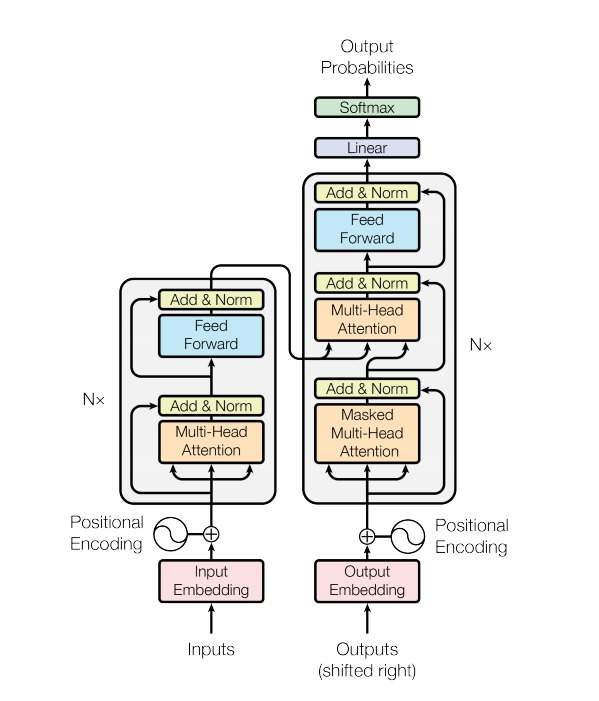
\includegraphics[width=0.68\linewidth]{images/transformer.png}
    \caption{Transformer model}
    \label{fig:transformer}
\end{figure}

\subsubsection{Positional encoding}

Attention layers see their input as a set of vectors, with no sequential order. This model also doesn't contain any recurrent or convolutional layers. Because of this a "positional encoding" is added to give the model some information about the relative position of the tokens in the sentence. \\
The positional encoding vector is added to the embedding vector. Embeddings represent a token in a d-dimensional space where tokens with similar meaning will be closer to each other. But the embeddings do not encode the relative position of tokens in a sentence. So after adding the positional encoding, tokens will be closer to each other based on the similarity of their meaning and their position in the sentence, in the d-dimensional space. The formula for calculating the positional encoding is as follows:

\[
    PE_{(pos, 2i)} = sin(pos/10000^{2i/d_{model}}), \qquad PE_{(pos, 2i+1)} = cos(pos/10000^{2i/d_{model}})
\]

\subsubsection{Self and multi-head attention}
The particular attention used by \cite{vaswani2017attention} is called "Scaled Dot-Product Attention" (Figure \ref{fig:transformer_attention} on the right). The input consists of queries and keys of dimension $dk$, and values of dimension $dv$. We compute the dot products of the query with all keys, divide each by $\sqrt{dk}$, and apply a softmax function to obtain the weights on the values.
\begin{figure}[H]%
    \centering
    \subfigure[Multi-Head Attention]{{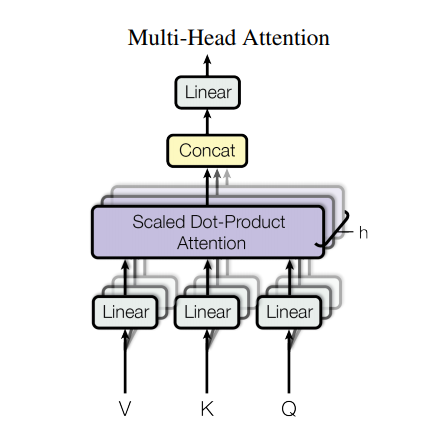
\includegraphics[width=0.4\linewidth]{images/multi_head_attention.png}}}%
    \subfigure[Scaled Dot-Product Attention]{{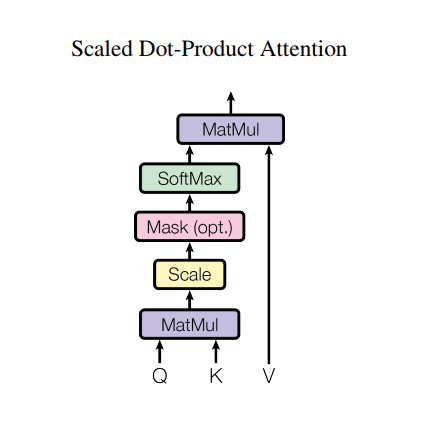
\includegraphics[width=0.4\linewidth]{images/self_attention.png}}}%
    \caption{On the left the multi-head attention is shown composed by multiple heads, on the right the single Scaled Dot-Product Attention mechanism.}
    \label{fig:transformer_attention}%
\end{figure}
The attention function is computed on a set of queries simultaneously, packed together into a matrix Q. The keys and values are also packed together into matrices K and V . We compute the matrix of outputs as:
%\begin{large}
$$Attention(Q, K, V ) = softmax(\frac{QK^T}{\sqrt{dk}})V$$
%\end{large}
Instead of performing a single attention function with keys, values and queries whose dimension is based on the model dimension, it is beneficial to linearly project the queries, keys and values h times with different, learned linear projections to dk, dk and dv dimensions, respectively. On each of these projected versions of queries, keys and values we then perform the attention function in parallel, yielding $dv$-dimensional output values. These are concatenated and once again projected, resulting in the final values, as depicted in Figure \ref{fig:transformer_attention} on the left.
Multi-head attention allows the model to jointly attend to information from different representation subspaces at different positions.

$$MultiHead(Q, K, V ) = Concat(head_{1}, ..., head_{h})W^O$$
where
$$head_{i} = Attention(QW^Q_{i}, KW^K_{i}, VW^V_{i})$$

If we call h as the number of parallel attention layers, or heads, for each of these we use $dk=dv=dmodel/h$ as dimension. Due to the reduced dimension of each head, the total computational cost is similar to that of single-head attention with full dimensionality.
\subsection{BERT and DistilBERT}\label{subsec:bert}
BERT (Bidirectional Encoder Representations from Transformers) is a multi-layer bidirectional Transformer encoder introduced by \cite{devlin2018bert} and  based on the original transformer implementation described in \cite{vaswani2017attention}.
\begin{figure}[H]%
    \centering
    \subfigure[BERT single layer]{{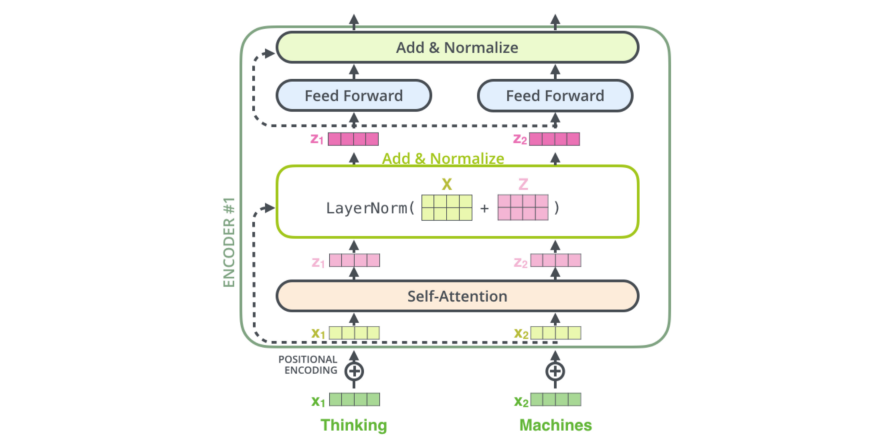
\includegraphics[width=0.50\linewidth]{images/bert_layer.png}}}%
    \subfigure[BERT stacked layers]{{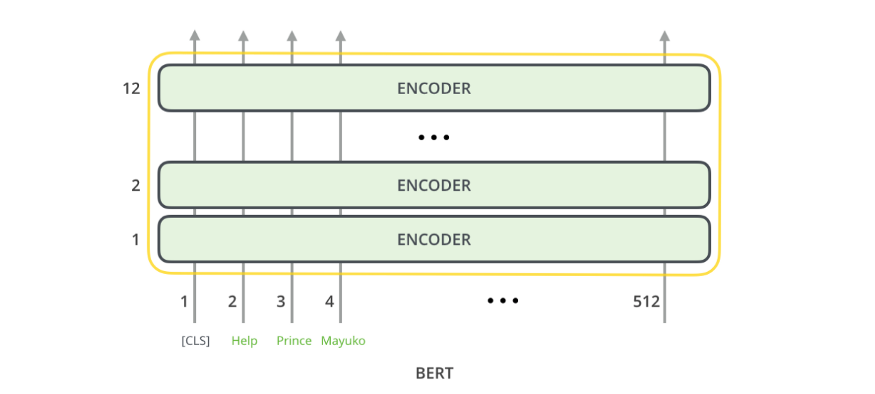
\includegraphics[width=0.50\linewidth]{images/bert_layers.png}}}%
    \caption{BERT architecture}
    \label{fig:bert}%
\end{figure}
BERT is conceptually simple and empirically powerful and that's why we decided to use it in our project, even though it's not aimed at NMT (its purpose are masked language tasks) it still provides great performances for our work, but BERT is extremely big even in his base form (it contains twelve layers, as many as a standar transformer) so it isn't the most cost-efficient model for our task, so for this reason we opted to use its distilled\footnote{Knowledge distillation is a compression technique in which a compact model - the student - is trained to reproduce the behaviour of a larger model - the teacher - or an ensemble of models.} version, called DistilBERT developed by \cite{sanh2019distilbert}.
\vspace{3mm}

DistilBERT is a small, fast, cheap and light Transformer model trained by distilling BERT. It has 40\% less parameters than BERT, runs 60\% faster while preserving over 95\% of BERT’s performances as measured on the GLUE language understanding benchmark from \cite{wang2018glue}. For those reasons, DistilBERT was chosen instead of BERT since we didn't have very powerful machines in our hands.

\subsection{RoBERTa}
Roberta is a transformer encoder with the same architecture as BERT, described in \ref{subsec:bert}, developed by Facebook AI. As written by \cite{liu2019roberta}, the team found that BERT was significantly undertrained, and can match or exceed the performance of every model published after it. They have just modified BERT key hyperparameters, removing the next-sentence pre-training objective and training with much larger mini-batches and learning rates. In 2019, when Facebook AI wrote the article, their best model achieved state-of-the-art results on GLUE (\cite{wang2018glue}), RACE and SQuAD.
\subsection{T5v11}
A Google research team published the paper by \cite{raffel2019exploring}, introducing a novel “Text-to-Text Transfer Transformer” (T5) transformer model which can convert any language problem into a text-to-text format.
\begin{figure}[H]
    \centering
    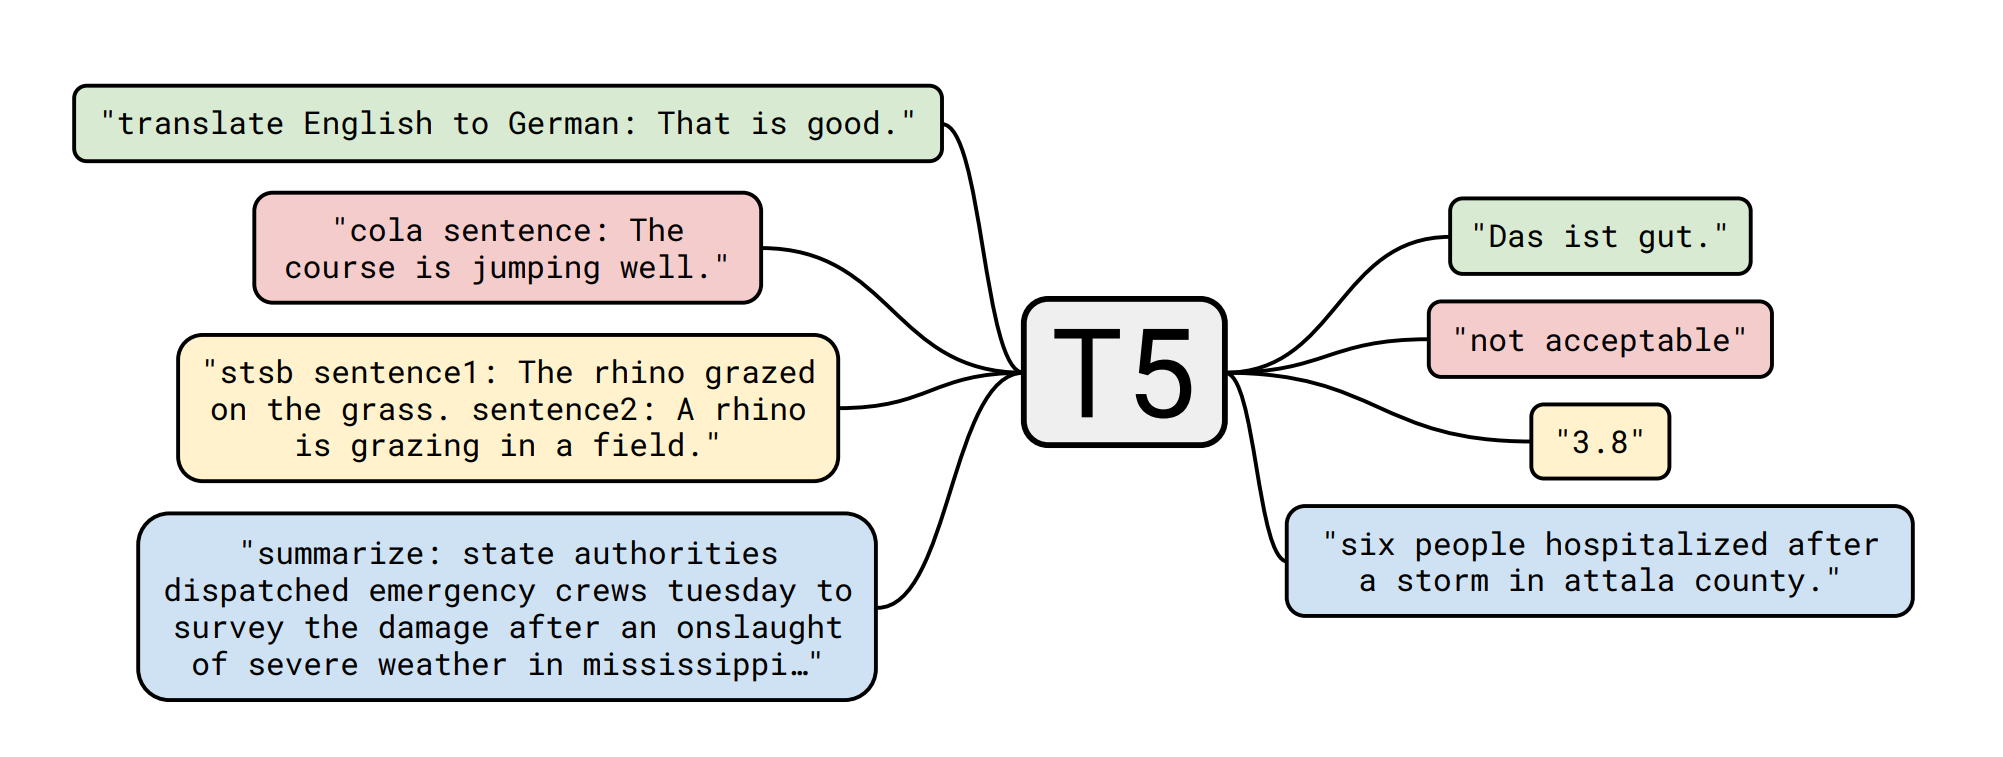
\includegraphics[width = .7\linewidth]{images/google_T5.png}
    \caption{Google T5 model.}
    \label{fig:google_t5}
\end{figure}
The idea behind T5 was to exploit the potential of transfer learning, where a model is first pre-trained on a data-rich task before being fine-tuned on a downstream task, emerging as a powerful technique in natural language processing (NLP). The proposed model is essentially a Encoder-Decoder Transformer with some architectural changes (like applying Layer Normalization before a sub block and then adding the initial input to the sub-block output; also known as pre-norm).
\vspace{3mm}

The model configuration is similar to BERT base and we decided to use the more polished version, T5v11, since it had some improvements:
\begin{itemize}
    \item GEGLU activation in the feed-forward hidden layer, rather than ReLU.
    \item Dropout was turned off in pre-training (quality win). Dropout should be re-enabled during fine-tuning (which we did).
    \item Pre-trained on C4 only without mixing in the downstream tasks.
    \item No parameter sharing between the embedding and classifier layer.
\end{itemize}
Between all the transformers models we considered for the project, T5 was the only one aimed at an NMT task, so we expected it to give us better performances than the previous models we've shown.